\documentclass[12pt]{article}
\usepackage{graphicx}
\usepackage{float}
\usepackage{amsmath}
\usepackage{amscd}
\usepackage{hyperref}
\usepackage{enumerate}
\usepackage{amsfonts}
\usepackage{amssymb}
\usepackage[utf8]{inputenc}
\usepackage{amsthm}
\usepackage{subcaption}
\usepackage{listings}
\usepackage{lscape}
\usepackage{tikz}
\usepackage{color} %red, green, blue, yellow, cyan, magenta, black, white
\usepackage{fullpage}
\usepackage{mathtools}
\usepackage{booktabs}
\usepackage{longtable}

\definecolor{mygreen}{RGB}{28,172,0} % color values Red, Green, Blue
\definecolor{mylilas}{RGB}{170,55,241}

\newtheorem{theorem}{Teorema}
\newtheorem{lem}[theorem]{Lemma}
\newtheorem{dfn}{Definición}
\newtheorem{cor}[theorem]{Corolario}
\newtheorem{obs}{Obs}
\newtheorem{rem}{Remark}
\newtheorem{prob}{Problema}

\newcommand*\circled[1]{\tikz[baseline=(char.base)]{
            \node[shape=circle,draw,inner sep=.05pt] (char) {#1};}}
            

\newtheoremstyle{named}{}{}{\itshape}{}{\bfseries}{.}{.5em} {\thmnote{#3 }#1}
\theoremstyle{named}
\newtheorem*{namedtheorem}{}


\newcounter{exercisecounter}
\newenvironment{ex}{\begin{quote}%
    \refstepcounter{exercisecounter}%
  \textbf{Ejercicio \arabic{exercisecounter}}%
  \quad
}{%
\end{quote}%
}
\newcounter{ejemplocounter}
\newenvironment{ej}{\begin{quote}%
    \refstepcounter{ejemplocounter}%
  \textbf{Ejemplo \arabic{ejemplocounter}}%
  \quad
}{%
\end{quote}%
}

\renewcommand{\d}[1]{\ensuremath{\operatorname{d}\!{#1}}}

\DeclarePairedDelimiter{\ceil}{\lceil}{\rceil}


\newcommand{\folder}{./Effect}

\begin{document}


\title{Treatment effects}

\author{Instituto Tecnológico Autónomo de México}
\date{\today}
\maketitle


\hrulefill


\section{Some Summary Statistics}

\vspace{7mm}

\subsection*{Administrative Stats}

Summary statistics of basic subject characteristics. All variables coming from casefile details are tested for balance between survey and non-survey populations.

\begin{center}
\scriptsize{
\begin{table}[!htbp] \centering 
  \caption{} 
  \label{} 
\begin{tabular}{@{\extracolsep{5pt}} cccccccc} 
\\[-1.8ex]\hline 
\hline \\[-1.8ex] 
Statistic & Treatment & Control & Treatment.1 & Control.1 & t-stat & Treatment.2 & Control.2 \\ 
\hline \\[-1.8ex] 
Wage & $1,522$ & $396$ & $620.698$ & $580.082$ & $0.797$ & $787.098$ & $930.839$ \\ 
Female & $1,522$ & $396$ & $0.445$ & $0.444$ & $0.013$ & $0.497$ & $0.498$ \\ 
Public Lawyer & $1,522$ & $396$ & $0.064$ & $0.071$ & $$-$0.486$ & $0.244$ & $0.257$ \\ 
Tenure & $1,522$ & $396$ & $3.898$ & $4.073$ & $$-$0.555$ & $5.299$ & $5.668$ \\ 
Bought durable goods recently & $170$ & $25$ & $0.082$ & $0.080$ & $$ & $0.276$ & $0.277$ \\ 
Working at the time & $172$ & $24$ & $0.465$ & $0.458$ & $$ & $0.500$ & $0.509$ \\ 
Looking for a job & $168$ & $24$ & $0.571$ & $0.500$ & $$ & $0.496$ & $0.511$ \\ 
\hline \\[-1.8ex] 
\end{tabular} 
\end{table} 
}
\end{center}


\pagebreak

\begin{center}
\scriptsize{% Table generated by Excel2LaTeX from sheet 'TAB_survey'
\begin{tabular}{rr}
\toprule
\multicolumn{2}{c}{Anger employee} \\
\midrule
\midrule
\multicolumn{1}{l}{A lot} & 127 \\
\multicolumn{1}{l}{Fairly} & 37 \\
\multicolumn{1}{l}{Little } & 15 \\
\multicolumn{1}{l}{Nothing} & 34 \\
\midrule
\multicolumn{2}{c}{Education employee} \\
\midrule
\midrule
\multicolumn{1}{l}{Elementary} & 15 \\
\multicolumn{1}{l}{Secondary} & 58 \\
\multicolumn{1}{l}{High-School} & 61 \\
\multicolumn{1}{l}{+ High School} & 79 \\
\midrule
\multicolumn{2}{c}{Cases employee's lawyer} \\
\midrule
\midrule
\multicolumn{1}{l}{1-10} & 93 \\
\multicolumn{1}{l}{11-30} & 114 \\
\multicolumn{1}{l}{31-100} & 222 \\
\multicolumn{1}{l}{+ 100} & 441 \\
\midrule
\multicolumn{2}{c}{Cases firm's lawyer} \\
\midrule
\midrule
\multicolumn{1}{l}{1-10} & 41 \\
\multicolumn{1}{l}{11-30} & 48 \\
\multicolumn{1}{l}{31-100} & 115 \\
\multicolumn{1}{l}{+ 100} & 328 \\
\bottomrule
\end{tabular}%
}
\end{center}

\pagebreak

\begin{landscape}
\begin{center}
\scriptsize{% Table generated by Excel2LaTeX from sheet 'ITT_ATT_report'
\begin{tabular}{lrrlllrrr}
      & \multicolumn{4}{c}{Conciliation} &       & \multicolumn{1}{c}{Calculator Plaintiff} & \multicolumn{1}{c}{Calculator Defendant} & \multicolumn{1}{c}{Calculator Both} \\
\cmidrule{2-9}      & \multicolumn{1}{c}{ITT} & \multicolumn{1}{c}{ITT} & \multicolumn{1}{c}{ATT (Plaintiff)} & \multicolumn{1}{c}{ATT  (Defendant)} & \multicolumn{1}{c}{ATT (Both)} & \multicolumn{3}{c}{First Stage} \\
\cmidrule{2-9}Treatment  & \multicolumn{1}{l}{0.0377*} & \multicolumn{1}{l}{0.0324***} &       &       &       & \multicolumn{1}{l}{0.679***} & \multicolumn{1}{l}{0.390***} & \multicolumn{1}{l}{0.292***} \\
      & \multicolumn{1}{l}{(0.0182)} & \multicolumn{1}{l}{(0.0109)} &       &       &       & \multicolumn{1}{l}{(0.0163)} & \multicolumn{1}{l}{(0.0173)} & \multicolumn{1}{l}{(0.0195)} \\
Calculator  & \multicolumn{1}{l}{} & \multicolumn{1}{l}{} & 0.0478** & 0.0831*** & 0.111** &       &       &  \\
(instrumented with ITT) & \multicolumn{1}{l}{} & \multicolumn{1}{l}{} & (0.0165) & (0.0280) & (0.0389) &       &       &  \\
Constant  & \multicolumn{1}{l}{0.0924***} & \multicolumn{1}{l}{0.0594***} & 0.0581*** & 0.0606*** & 0.0605*** & \multicolumn{1}{l}{0.0282} & \multicolumn{1}{l}{-0.0143} & \multicolumn{1}{l}{-0.00946} \\
      & \multicolumn{1}{l}{(0.0129)} & \multicolumn{1}{l}{(0.0145)} & (0.0149) & (0.0142) & (0.0144) & \multicolumn{1}{l}{(0.0298)} & \multicolumn{1}{l}{(0.0183)} & \multicolumn{1}{l}{(0.0189)} \\
      &       &       &       &       &       &       &       &  \\
\midrule
Observations & \multicolumn{1}{l}{3114} & \multicolumn{1}{l}{3114} & 3114  & 3114  & 3114  & \multicolumn{1}{l}{3114} & \multicolumn{1}{l}{3114} & \multicolumn{1}{l}{3114} \\
Dummy subcourts & \multicolumn{1}{l}{NO} & \multicolumn{1}{l}{YES} & YES   & YES   & YES   & \multicolumn{1}{l}{YES} & \multicolumn{1}{l}{YES} & \multicolumn{1}{l}{YES} \\
R-squared & \multicolumn{1}{l}{0.00281} & \multicolumn{1}{l}{0.0339} & 0.0349 & 0.0603 & 0.0584 & \multicolumn{1}{l}{0.384} & \multicolumn{1}{l}{0.156} & \multicolumn{1}{l}{0.107} \\
DepVarMean & \multicolumn{1}{l}{0.119} & \multicolumn{1}{l}{0.119} & 0.119 & 0.119 & 0.119 & \multicolumn{1}{l}{0.500} & \multicolumn{1}{l}{0.290} & \multicolumn{1}{l}{0.290} \\
\% Treated &       &       & 0.500 & 0.290 & 0.221 &       &       &  \\
\bottomrule
\bottomrule
\end{tabular}%
}
\end{center}

\end{landscape}

\subsection*{Expectation Stats}

Summary statistics for expectations.

\begin{center}
\scriptsize{
\begin{table}[!htbp] \centering 
  \caption{} 
  \label{} 
\begin{tabular}{@{\extracolsep{5pt}}lccccc} 
\\[-1.8ex]\hline 
\hline \\[-1.8ex] 
Statistic & \multicolumn{1}{c}{N} & \multicolumn{1}{c}{Mean} & \multicolumn{1}{c}{St. Dev.} & \multicolumn{1}{c}{Min} & \multicolumn{1}{c}{Max} \\ 
\hline \\[-1.8ex] 
Payment prob. (baseline) & 248 & 78.782 & 24.885 & 10 & 100 \\ 
Payment amount (baseline) & 210 & 69,297.190 & 104,987.700 & 0.000 & 850,000.000 \\ 
Payment prob. (exit) & 186 & 70.452 & 28.466 & 10 & 100 \\ 
Payment amount (exit) & 157 & 58,355.640 & 73,370.290 & 0.000 & 500,000.000 \\ 
\hline \\[-1.8ex] 
\end{tabular} 
\end{table} 
}
\end{center}

\pagebreak

\subsection*{Update in beliefs}

The update in beliefs is measured in relative terms, this is the percentage deviation of the exit survey with respect to the entrance survey
\[\frac{exit-initial}{initial}\]

We provide two measures: Update in beliefs in probability and payment.\\

\begin{center}
\scriptsize{
\begin{table}[htbp]\centering \caption{Update in beleifs \label{sumstat}}
\begin{tabular}{l c c c c c}\hline\hline
\multicolumn{1}{c}{\textbf{Variable}} & \textbf{Mean}
 & \textbf{Std. Dev.}& \textbf{Min.} &  \textbf{Max.} & \textbf{N}\\ \hline
update\_emp\_fir\_law & -0.026 & 1.171 & -1 & 9 & 180\\
update\_emp & -0.106 & 0.578 & -1 & 2.2 & 70\\
update\_emp\_law & -0.216 & 0.560 & -1 & 1.875 & 210\\
\hline\end{tabular}
\end{table}
}
\end{center}

\begin{figure}[H]
\label{diff}
\begin{center}
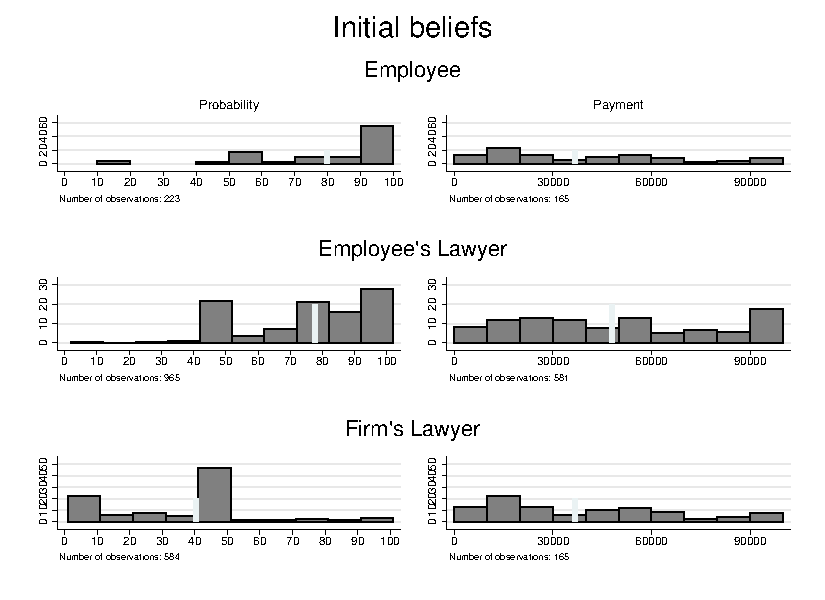
\includegraphics[width=\textwidth]{./Figures/belief.pdf}
\end{center}
{\footnotesize \textit{The histograms are trimmed at the 75 percentile in the case for amount. Width of bins are \$30,000 pesos for the case of amount and 10\% for the case of probability.}}
\end{figure}


\begin{figure}[H]
\label{update}
\begin{center}
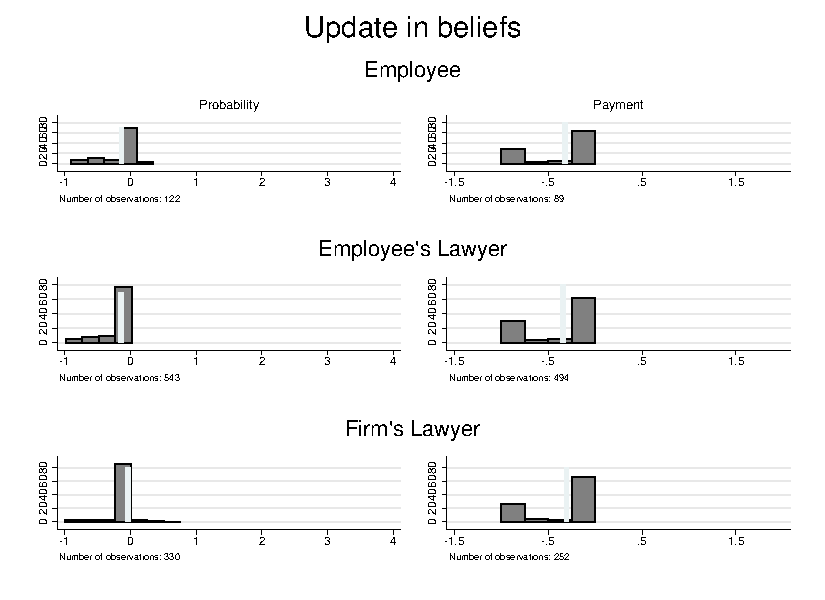
\includegraphics[width=\textwidth]{./Figures/update_belief.pdf}
\end{center}
{\footnotesize \textit{The histograms measures the update in relative terms. It displays the distribution from the percentile 5 to 95.}}
\end{figure}

\pagebreak


\begin{figure}[H]
\label{update}
\begin{center}
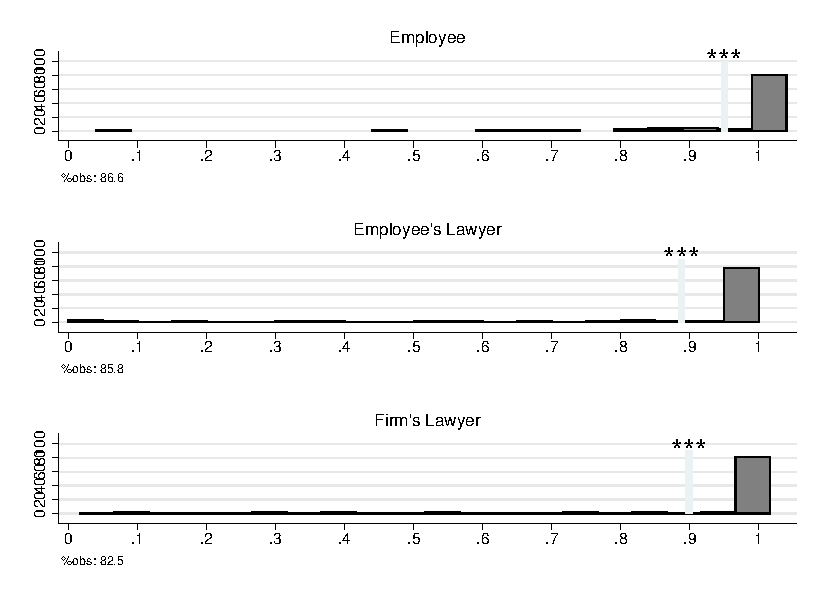
\includegraphics[width=\textwidth]{./Figures/updatebeleif_amount.pdf}
\end{center}
{\footnotesize \textit{Notes: Graphs on belief updating. They show the following statistic: $\theta=\left|\frac{P-exitsurvey}{P-initialsurvey}\right|$. Where $P$ is the prediction made by the calculator and $exit$ and $initial$ survey variables denote what each part answered on the survey for amount won. Note that when $\theta=1$ we have no update with respect to the prediction. And when $\theta<1$ they update in the direction of what calculator says. The extreme case $\theta=0$ implies perfect updating with respect to what the calculator says. }}
{\footnotesize \textit{Do file: } \texttt{Update\_beleifs.do}}
\end{figure}


\pagebreak

The following table displays a regression of conciliation against the statistics of updating
\[\theta=\left|\frac{P-exitsurvey}{P-initialsurvey}\right|\]

\begin{center}
\scriptsize{% Table generated by Excel2LaTeX from sheet 'con_vs_update'
\begin{tabular}{lcccccc}
      & \multicolumn{6}{c}{Conciliation } \\
\midrule
      & \multicolumn{2}{c}{Employee} & \multicolumn{2}{c}{Employee's Lawyer} & \multicolumn{2}{c}{Firm's Lawyer} \\
\midrule
\midrule
Update in beleifs & \multicolumn{1}{l}{0.341**} & \multicolumn{1}{l}{0.0389} & \multicolumn{1}{l}{-0.0499} & \multicolumn{1}{l}{-0.0108} & \multicolumn{1}{l}{0.00390} & \multicolumn{1}{l}{0.0158} \\
      & \multicolumn{1}{l}{(0.119)} & \multicolumn{1}{l}{(0.0664)} & \multicolumn{1}{l}{(0.0689)} & \multicolumn{1}{l}{(0.0507)} & \multicolumn{1}{l}{(0.0895)} & \multicolumn{1}{l}{(0.0714)} \\
Employee present (EP) & \multicolumn{1}{l}{} & \multicolumn{1}{l}{-0.384**} & \multicolumn{1}{l}{} & \multicolumn{1}{l}{0.395*} & \multicolumn{1}{l}{} & \multicolumn{1}{l}{0.947***} \\
      & \multicolumn{1}{l}{} & \multicolumn{1}{l}{(0.171)} & \multicolumn{1}{l}{} & \multicolumn{1}{l}{(0.211)} & \multicolumn{1}{l}{} & \multicolumn{1}{l}{(0.191)} \\
EP\#\#Update in beleifs & \multicolumn{1}{l}{} & \multicolumn{1}{l}{0.673***} & \multicolumn{1}{l}{} & \multicolumn{1}{l}{-0.255} & \multicolumn{1}{l}{} & \multicolumn{1}{l}{-0.736***} \\
      & \multicolumn{1}{l}{} & \multicolumn{1}{l}{(0.191)} & \multicolumn{1}{l}{} & \multicolumn{1}{l}{(0.237)} & \multicolumn{1}{l}{} & \multicolumn{1}{l}{(0.195)} \\
Constant  & \multicolumn{1}{l}{-0.0997} & \multicolumn{1}{l}{0.0273} & \multicolumn{1}{l}{0.179**} & \multicolumn{1}{l}{0.121**} & \multicolumn{1}{l}{0.196*} & \multicolumn{1}{l}{0.139} \\
      & \multicolumn{1}{l}{(0.0925)} & \multicolumn{1}{l}{(0.0607)} & \multicolumn{1}{l}{(0.0658)} & \multicolumn{1}{l}{(0.0526)} & \multicolumn{1}{l}{(0.0974)} & \multicolumn{1}{l}{(0.0809)} \\
      &       &       &       &       &       &  \\
\midrule
Observations & \multicolumn{1}{l}{120} & \multicolumn{1}{l}{120} & \multicolumn{1}{l}{478} & \multicolumn{1}{l}{478} & \multicolumn{1}{l}{301} & \multicolumn{1}{l}{301} \\
R-squared & \multicolumn{1}{l}{0.0151} & \multicolumn{1}{l}{0.120} & \multicolumn{1}{l}{0.00135} & \multicolumn{1}{l}{0.0343} & \multicolumn{1}{l}{0.00000552} & \multicolumn{1}{l}{0.0685} \\
Update var mean & \multicolumn{2}{c}{0.954} & \multicolumn{2}{c}{0.895} & \multicolumn{2}{c}{0.914} \\
\bottomrule
\bottomrule
\end{tabular}%
}
\end{center}


\pagebreak


Now we test difference in initial and exit survey in expectations. The following table shows the results.

\begin{center}
\scriptsize{% Table generated by Excel2LaTeX from sheet 'ttest'
\begin{tabular}{rrrr}
\toprule
      & \multicolumn{1}{c}{Initial} & \multicolumn{1}{c}{Exit} & \multicolumn{1}{c}{p-value} \\
\midrule
\multicolumn{4}{c}{Probability} \\
\midrule
\midrule
Employee  & \multicolumn{1}{l}{79.927} & \multicolumn{1}{l}{71.945} & \multicolumn{1}{l}{0} \\
      & \multicolumn{1}{l}{(24.703)} & \multicolumn{1}{l}{(28.661)} & \multicolumn{1}{l}{} \\
Employees Lawyer & \multicolumn{1}{l}{77.007} & \multicolumn{1}{l}{67.658} & \multicolumn{1}{l}{0} \\
      & \multicolumn{1}{l}{(20.208)} & \multicolumn{1}{l}{(24.383)} & \multicolumn{1}{l}{} \\
Firms Lawyer & \multicolumn{1}{l}{40.822} & \multicolumn{1}{l}{42.267} & \multicolumn{1}{l}{0.122} \\
      & \multicolumn{1}{l}{(23.101)} & \multicolumn{1}{l}{(23.24)} & \multicolumn{1}{l}{} \\
      \midrule
\multicolumn{4}{c}{Payment levels} \\
\midrule
\midrule
Employee  & \multicolumn{1}{l}{54344.478} & \multicolumn{1}{l}{54930.941} & \multicolumn{1}{l}{0.804} \\
      & \multicolumn{1}{l}{(64865.672)} & \multicolumn{1}{l}{(66475.18)} & \multicolumn{1}{l}{} \\
Employees Lawyer & \multicolumn{1}{l}{97829.594} & \multicolumn{1}{l}{88209.612} & \multicolumn{1}{l}{0} \\
      & \multicolumn{1}{l}{(108525.677)} & \multicolumn{1}{l}{(97808.871)} & \multicolumn{1}{l}{} \\
Firms Lawyer & \multicolumn{1}{l}{56229.145} & \multicolumn{1}{l}{54309.441} & \multicolumn{1}{l}{0.564} \\
      & \multicolumn{1}{l}{(74573.935)} & \multicolumn{1}{l}{(67685.482)} & \multicolumn{1}{l}{} \\
      \midrule
\multicolumn{4}{c}{Payment logs} \\
\midrule
\midrule
Employee  & \multicolumn{1}{l}{10.219} & \multicolumn{1}{l}{10.269} & \multicolumn{1}{l}{0.454} \\
      & \multicolumn{1}{l}{(1.709)} & \multicolumn{1}{l}{(1.617)} & \multicolumn{1}{l}{} \\
Employees Lawyer & \multicolumn{1}{l}{10.855} & \multicolumn{1}{l}{10.771} & \multicolumn{1}{l}{0.002} \\
      & \multicolumn{1}{l}{(1.569)} & \multicolumn{1}{l}{(1.523)} & \multicolumn{1}{l}{} \\
Firms Lawyer & \multicolumn{1}{l}{9.422} & \multicolumn{1}{l}{9.483} & \multicolumn{1}{l}{0.554} \\
      & \multicolumn{1}{l}{(3.303)} & \multicolumn{1}{l}{(3.117)} & \multicolumn{1}{l}{} \\
\bottomrule
\end{tabular}%
}
\end{center}

\pagebreak

\section{ITT and ATT regressions}

\begin{landscape}
\subsection*{ITT and Second Stage ATT}

\begin{center}
\scriptsize{% Table generated by Excel2LaTeX from sheet 'ITT_ATT'
\begin{tabular}{lrrlrlrlrrr}
      & \multicolumn{7}{c}{Conciliation}                      & \multicolumn{1}{c}{Calculator Plaintiff} & \multicolumn{1}{c}{Calculator Defendant} & \multicolumn{1}{c}{Calculator Both} \\
\cmidrule{2-11}      & \multicolumn{1}{c}{ITT} & \multicolumn{1}{c}{ITT} & \multicolumn{2}{c}{ATT (Plaintiff)} & \multicolumn{2}{c}{ATT  (Defendant)} & \multicolumn{1}{c}{ATT (Both)} & \multicolumn{3}{c}{First Stage} \\
\cmidrule{2-11}Treatment  & \multicolumn{1}{l}{0.0540*} & \multicolumn{1}{l}{0.0486**} &       &       &       &       &       & \multicolumn{1}{l}{0.722***} & \multicolumn{1}{l}{0.635***} & \multicolumn{1}{l}{0.489***} \\
      & \multicolumn{1}{l}{(0.0264)} & \multicolumn{1}{l}{(0.0202)} &       &       &       &       &       & \multicolumn{1}{l}{(0.0215)} & \multicolumn{1}{l}{(0.0220)} & \multicolumn{1}{l}{(0.0263)} \\
Calculator  & \multicolumn{1}{l}{} & \multicolumn{1}{l}{} & 0.0673** &       & 0.0766** &       & 0.0995** &       &       &  \\
(instrumented with ITT) & \multicolumn{1}{l}{} & \multicolumn{1}{l}{} & (0.0281) &       & (0.0317) &       & (0.0417) &       &       &  \\
Calculator  &       &       &       & \multicolumn{1}{l}{-0.0141} &       & \multicolumn{1}{l}{-0.0158} &       &       &       &  \\
(instrumented with ITT \& ITT*EP) &       &       &       & \multicolumn{1}{l}{(0.0249)} &       & \multicolumn{1}{l}{(0.0286)} &       &       &       &  \\
Constant  & \multicolumn{1}{l}{0.159***} & \multicolumn{1}{l}{0.124***} & 0.123*** & \multicolumn{1}{l}{0.131***} & 0.125*** & \multicolumn{1}{l}{0.129***} & 0.125*** & \multicolumn{1}{l}{0.0150} & \multicolumn{1}{l}{-0.0150} & \multicolumn{1}{l}{-0.00841} \\
      & \multicolumn{1}{l}{(0.0184)} & \multicolumn{1}{l}{(0.0286)} & (0.0293) & \multicolumn{1}{l}{(0.0269)} & (0.0273) & \multicolumn{1}{l}{(0.0268)} & (0.0280) & \multicolumn{1}{l}{(0.0319)} & \multicolumn{1}{l}{(0.0289)} & \multicolumn{1}{l}{(0.0287)} \\
      &       &       &       &       &       &       &       &       &       &  \\
\midrule
Observations & \multicolumn{1}{l}{1285} & \multicolumn{1}{l}{1285} & 1285  & \multicolumn{1}{l}{1285} & 1285  & \multicolumn{1}{l}{1285} & 1285  & \multicolumn{1}{l}{1285} & \multicolumn{1}{l}{1285} & \multicolumn{1}{l}{1285} \\
Dummy subcourts & \multicolumn{1}{l}{NO} & \multicolumn{1}{l}{YES} & YES   & \multicolumn{1}{l}{YES} & YES   & \multicolumn{1}{l}{YES} & YES   & \multicolumn{1}{l}{YES} & \multicolumn{1}{l}{YES} & \multicolumn{1}{l}{YES} \\
Conditioning on notified & \multicolumn{1}{l}{YES} & \multicolumn{1}{l}{YES} & YES   & \multicolumn{1}{l}{YES} & YES   & \multicolumn{1}{l}{YES} & YES   & \multicolumn{1}{l}{YES} & \multicolumn{1}{l}{YES} & \multicolumn{1}{l}{YES} \\
R-squared & \multicolumn{1}{l}{0.00392} & \multicolumn{1}{l}{0.0449} & 0.0457 & \multicolumn{1}{l}{0.0905} & 0.0500 & \multicolumn{1}{l}{0.102} & 0.0494 & \multicolumn{1}{l}{0.448} & \multicolumn{1}{l}{0.343} & \multicolumn{1}{l}{0.222} \\
DepVarMean & \multicolumn{1}{l}{0.197} & \multicolumn{1}{l}{0.197} & 0.197 & \multicolumn{1}{l}{0.197} & 0.197 & \multicolumn{1}{l}{0.197} & 0.197 & \multicolumn{1}{l}{0.519} & \multicolumn{1}{l}{0.453} & \multicolumn{1}{l}{0.453} \\
\% Treated &       &       & 0.519 &       & 0.453 &       & 0.355 &       &       &  \\
\bottomrule
\bottomrule
\end{tabular}%
}
\end{center}

\end{landscape}

\pagebreak


\subsection*{First Stage for ATT regressions}

\begin{center}
\scriptsize{% Table generated by Excel2LaTeX from sheet 'FS_ATT'
\begin{tabular}{rrrrrrr}
\toprule
      & \multicolumn{3}{c}{Plaintiff} & \multicolumn{3}{c}{Defendant} \\
\midrule
      & \multicolumn{1}{c}{Calculator} & \multicolumn{1}{c}{Calculator} & \multicolumn{1}{c}{Calculator*EP} & \multicolumn{1}{c}{Calculator} & \multicolumn{1}{c}{Calculator} & \multicolumn{1}{c}{Calculator*EP} \\
ITT   & \multicolumn{1}{l}{0.679***} & \multicolumn{1}{l}{0.648***} & \multicolumn{1}{l}{-0.000286} & \multicolumn{1}{l}{0.395***} & \multicolumn{1}{l}{0.381***} & \multicolumn{1}{l}{0.00219} \\
      & \multicolumn{1}{l}{(0.0112)} & \multicolumn{1}{l}{(0.0123)} & \multicolumn{1}{l}{(0.00164)} & \multicolumn{1}{l}{(0.0119)} & \multicolumn{1}{l}{(0.0126)} & \multicolumn{1}{l}{(0.00234)} \\
ITT*EP & \multicolumn{1}{l}{} & \multicolumn{1}{l}{0.192***} & \multicolumn{1}{l}{0.861***} & \multicolumn{1}{l}{} & \multicolumn{1}{l}{0.0837***} & \multicolumn{1}{l}{0.488***} \\
      & \multicolumn{1}{l}{} & \multicolumn{1}{l}{(0.0214)} & \multicolumn{1}{l}{(0.0184)} & \multicolumn{1}{l}{} & \multicolumn{1}{l}{(0.0258)} & \multicolumn{1}{l}{(0.0257)} \\
Court 7 & \multicolumn{1}{l}{0.00758} & \multicolumn{1}{l}{0.00426} & \multicolumn{1}{l}{0.00101} & \multicolumn{1}{l}{0.0201} & \multicolumn{1}{l}{0.0186} & \multicolumn{1}{l}{0.00304} \\
      & \multicolumn{1}{l}{(0.0227)} & \multicolumn{1}{l}{(0.0224)} & \multicolumn{1}{l}{(0.00619)} & \multicolumn{1}{l}{(0.0228)} & \multicolumn{1}{l}{(0.0228)} & \multicolumn{1}{l}{(0.00997)} \\
Court 9 & \multicolumn{1}{l}{-0.0317} & \multicolumn{1}{l}{-0.0331} & \multicolumn{1}{l}{-0.0106} & \multicolumn{1}{l}{0.00543} & \multicolumn{1}{l}{0.00482} & \multicolumn{1}{l}{-0.00495} \\
      & \multicolumn{1}{l}{(0.0232)} & \multicolumn{1}{l}{(0.0229)} & \multicolumn{1}{l}{(0.00722)} & \multicolumn{1}{l}{(0.0227)} & \multicolumn{1}{l}{(0.0227)} & \multicolumn{1}{l}{(0.00977)} \\
Court 11 & \multicolumn{1}{l}{-0.00328} & \multicolumn{1}{l}{0.000422} & \multicolumn{1}{l}{-0.0103} & \multicolumn{1}{l}{0.0660***} & \multicolumn{1}{l}{0.0676***} & \multicolumn{1}{l}{0.00966} \\
      & \multicolumn{1}{l}{(0.0225)} & \multicolumn{1}{l}{(0.0224)} & \multicolumn{1}{l}{(0.00661)} & \multicolumn{1}{l}{(0.0229)} & \multicolumn{1}{l}{(0.0228)} & \multicolumn{1}{l}{(0.00916)} \\
Court 16 & \multicolumn{1}{l}{-0.0261} & \multicolumn{1}{l}{-0.0289} & \multicolumn{1}{l}{0.00403} & \multicolumn{1}{l}{0.00389} & \multicolumn{1}{l}{0.00266} & \multicolumn{1}{l}{0.00973} \\
      & \multicolumn{1}{l}{(0.0230)} & \multicolumn{1}{l}{(0.0225)} & \multicolumn{1}{l}{(0.00600)} & \multicolumn{1}{l}{(0.0226)} & \multicolumn{1}{l}{(0.0224)} & \multicolumn{1}{l}{(0.0102)} \\
Notified & \multicolumn{1}{l}{0.0512***} & \multicolumn{1}{l}{0.0436***} & \multicolumn{1}{l}{0.0104**} & \multicolumn{1}{l}{0.286***} & \multicolumn{1}{l}{0.282***} & \multicolumn{1}{l}{0.0624***} \\
      & \multicolumn{1}{l}{(0.0141)} & \multicolumn{1}{l}{(0.0140)} & \multicolumn{1}{l}{(0.00445)} & \multicolumn{1}{l}{(0.0147)} & \multicolumn{1}{l}{(0.0147)} & \multicolumn{1}{l}{(0.00631)} \\
Constant  & \multicolumn{1}{l}{0.00775} & \multicolumn{1}{l}{0.0120} & \multicolumn{1}{l}{0.000434} & \multicolumn{1}{l}{-0.128***} & \multicolumn{1}{l}{-0.126***} & \multicolumn{1}{l}{-0.0293***} \\
      & \multicolumn{1}{l}{(0.0178)} & \multicolumn{1}{l}{(0.0175)} & \multicolumn{1}{l}{(0.00449)} & \multicolumn{1}{l}{(0.0179)} & \multicolumn{1}{l}{(0.0179)} & \multicolumn{1}{l}{(0.00746)} \\
      & \multicolumn{1}{l}{} & \multicolumn{1}{l}{} & \multicolumn{1}{l}{} & \multicolumn{1}{l}{} & \multicolumn{1}{l}{} & \multicolumn{1}{l}{} \\
Observations & \multicolumn{1}{l}{3114} & \multicolumn{1}{l}{3114} & \multicolumn{1}{l}{3114} & \multicolumn{1}{l}{3114} & \multicolumn{1}{l}{3114} & \multicolumn{1}{l}{3114} \\
R-squared & \multicolumn{1}{l}{0.387} & \multicolumn{1}{l}{0.401} & \multicolumn{1}{l}{0.842} & \multicolumn{1}{l}{0.252} & \multicolumn{1}{l}{0.255} & \multicolumn{1}{l}{0.476} \\
\bottomrule
\end{tabular}%
}
\end{center}


\section{Take up regression (calculator and survey)}


\begin{center}
\scriptsize{% Table generated by Excel2LaTeX from sheet 'Take_up'
\begin{tabular}{rrrrr}
\toprule
      & \multicolumn{2}{c}{Calculator} & \multicolumn{2}{c}{Survey} \\
\midrule
      & \multicolumn{1}{c}{Plaintiff} & \multicolumn{1}{c}{Defendant} & \multicolumn{1}{c}{Plaintiff} & \multicolumn{1}{c}{Defendant} \\
      &       &       &       &  \\
Female & \multicolumn{1}{l}{-0.0232} & \multicolumn{1}{l}{0.00164} & \multicolumn{1}{l}{-0.0178} & \multicolumn{1}{l}{-0.0154} \\
      & \multicolumn{1}{l}{(0.0210)} & \multicolumn{1}{l}{(0.0219)} & \multicolumn{1}{l}{(0.0233)} & \multicolumn{1}{l}{(0.0219)} \\
c\_antiguedad & \multicolumn{1}{l}{-0.00108} & \multicolumn{1}{l}{0.00266} & \multicolumn{1}{l}{-0.00244} & \multicolumn{1}{l}{0.000392} \\
      & \multicolumn{1}{l}{(0.00191)} & \multicolumn{1}{l}{(0.00197)} & \multicolumn{1}{l}{(0.00206)} & \multicolumn{1}{l}{(0.00195)} \\
c\_indem & \multicolumn{1}{l}{-0.000000141} & \multicolumn{1}{l}{-4.80e-08} & \multicolumn{1}{l}{-0.000000143} & \multicolumn{1}{l}{-8.74e-08} \\
      & \multicolumn{1}{l}{(0.000000131)} & \multicolumn{1}{l}{(0.000000131)} & \multicolumn{1}{l}{(0.000000152)} & \multicolumn{1}{l}{(0.000000145)} \\
dummy\_reinst & \multicolumn{1}{l}{0.00179} & \multicolumn{1}{l}{0.0162} & \multicolumn{1}{l}{0.0150} & \multicolumn{1}{l}{0.0439*} \\
      & \multicolumn{1}{l}{(0.0218)} & \multicolumn{1}{l}{(0.0227)} & \multicolumn{1}{l}{(0.0241)} & \multicolumn{1}{l}{(0.0228)} \\
Public Lawyer & \multicolumn{1}{l}{0.00118} & \multicolumn{1}{l}{0.00459} & \multicolumn{1}{l}{-0.0436*} & \multicolumn{1}{l}{-0.0117} \\
      & \multicolumn{1}{l}{(0.0211)} & \multicolumn{1}{l}{(0.0222)} & \multicolumn{1}{l}{(0.0240)} & \multicolumn{1}{l}{(0.0213)} \\
Constant  & \multicolumn{1}{l}{0.696***} & \multicolumn{1}{l}{0.378***} & \multicolumn{1}{l}{0.638***} & \multicolumn{1}{l}{0.310***} \\
      & \multicolumn{1}{l}{(0.0332)} & \multicolumn{1}{l}{(0.0349)} & \multicolumn{1}{l}{(0.0378)} & \multicolumn{1}{l}{(0.0341)} \\
      & \multicolumn{1}{l}{} & \multicolumn{1}{l}{} & \multicolumn{1}{l}{} & \multicolumn{1}{l}{} \\
Observations & \multicolumn{1}{l}{2066} & \multicolumn{1}{l}{2066} & \multicolumn{1}{l}{1862} & \multicolumn{1}{l}{1830} \\
R-squared & \multicolumn{1}{l}{0.00125} & \multicolumn{1}{l}{0.00120} & \multicolumn{1}{l}{0.00346} & \multicolumn{1}{l}{0.00286} \\
Dep Var Mean & \multicolumn{1}{l}{0.676} & \multicolumn{1}{l}{0.399} & \multicolumn{1}{l}{0.570} & \multicolumn{1}{l}{0.308} \\
\bottomrule
\end{tabular}%
}
\end{center}


%%%%%%%%%%%%%%%%%%%%%%%%%%%%%%%%%%%%%%%%%%%%%%%%%%%%%%%%%%%%%%%%%%%%%%%%%%%%%%%%
\end{document}
